\chapter*{Исполнитель Кузнечик}
\addtocounter{chapter}{1}

\section{Общие сведения}

\subsection{Цель разработки и содержимое поставки}
Цель разработки --- создание исполнителя Кузнечик в соответствии с учебником «Инфор\-ма\-тика-6». Настоящая поставка содержит исполнитель, который может работать как в автономном режиме, так и под управлением системы КуМир.

\subsection{Платформа разработки}
Как и система Кумир 1.7.0, исполнитель Кузнечик  разрабатывается с помощью библиотеки классов Qt-4 и, таким образом, является кросс-платформенной разработкой. В настоящее время созданы версии для Windows и Linux. 

\subsection{Описание поставки. Инсталляция}
В поставку системы КуМир (версия 03.11.09 и позднее) входят как собственно система Кумир, так и ряд исполнителей. Каждый такой исполнитель может использоваться как внутри системы КуМир, так и автономно.

\subsection{Запуск исполнителя}
Необходимо инсталлировать систему КуМир (версия 03.11.09 и позднее). Исполнитель входит в поставку и запускается автоматически. Для использования в программе алгоритмов Кузнечика необходимо написать в программе \textsf{использовать Кузнечик}.

Для запуска Кузнечика в автономном режиме нужно нажать иконку «Кузнечик» в меню программ. Эта иконка создается при инсталляции системы КуМир и при необходимости может быть перенесена на рабочий стол.

\section{Описание работы исполнителя}

\subsection{Окна}

При запуске исполнителя создаются два окна (см.~\ref{kuznechik}):
\begin{itemize}
\item окно Кузнечика;
\item окно пульта.
\end{itemize}
\begin{figure}[h]
	\begin{center}
		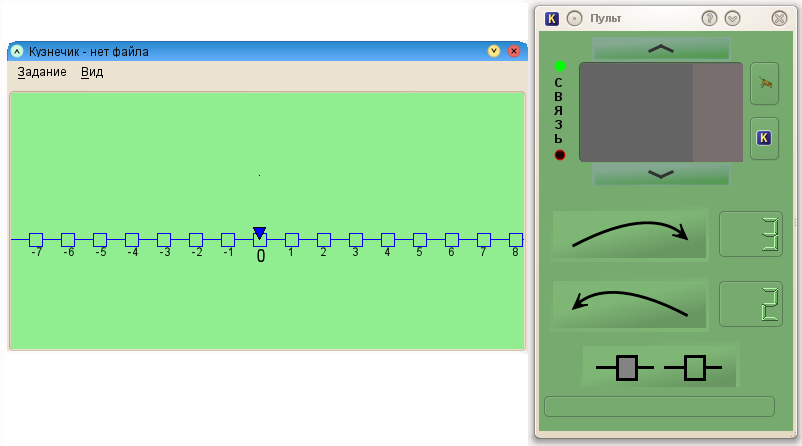
\includegraphics[scale=0.6]{kuznechik.png}
	\end{center}
	\caption{Окно Кузнечика и пульт}
\label{kuznechik}
\end{figure}

Окна пульта и кузнечика --- стандартные окна операционной системы. Их можно передвигать по экрану, сворачивать и разворачивать обычным образом. Ограничения: размер пульта менять нельзя; размер окна кузнечика можно менять только в ширину. 


\subsection{Окно Кузнечика}

Окно кузнечика – прямоугольное. Оно содержит:
\begin{itemize}
\item рабочее поле, на котором показана числовая ось, кузнечик (в виде треугольника, см.~\ref{kuznechik});
\item меню «Задание»;
\item меню «Вид».
\end{itemize}

Меню «Задание» описано ниже. Меню «Вид» позволяет менять масштаб изображения. Это же можно делать, используя колесико мышки (вверх --- крупнее, вниз --- мельче). Мышкой можно «протягивать» в окне бесконечное влево и вправо поле кузнечика. Кроме того меню «Вид» содержит строку «Найти кузнечика». Это действие сдвигает область видимости так, чтобы Кузнечик оказался в центре экрана. Масштаб при этом не меняется.

\subsection{Задания кузнечика}
Задание кузнечика включает описание:
\begin{enumerate}
\item длины прыжков вперед и назад (два натуральных числа);
\item начального положения;
\item описание области, доступной Кузнечику (может отсутствовать);
\item флагов (могут отсутствовать).
\end{enumerate}

Длины прыжков показаны на пульте (рядом со стрелками). Если целевое положение задано, соответствующая позиция показано флажком. Когда кузнечик попадает в  это положение, цвет флажка меняется. Если заданы границы доступной Кузнечику области, то соответствующая часть числовой прямой отделяется красными линиями.

Для выбора задания используется меню «Задание» окна Кузнечика. В нем есть пункты «Новое», «Загрузить», «Сохранить». Пункт «Новое» вызывает появление окна установки задания (см.~\ref{kuznechik-task}). Пункты «Загрузить» и «Сохранить» работают стандартным образом.


\begin{figure}[h]
	\begin{center}
		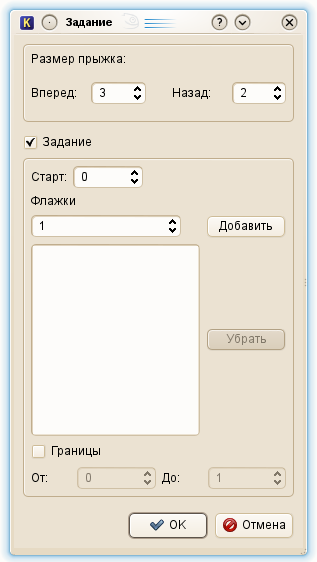
\includegraphics[scale=0.6]{kuznechik-task.png}
	\end{center}
	\caption{Окно установки задания Кузнечика}
\label{kuznechik-task}
\end{figure}

\subsection{Окно пульта}
Окно пульта содержит:
\begin{itemize}
\item поле протоколирования команд (бесконечное вниз) и кнопки прокрутки протокола (сверху и снизу от поля);
\item кнопку сброса (справа от протокола вверху); при нажатии этой кнопки арена сбрасывается в начальное положение, а поле протокола очищается;
\item кнопку передачи протокола в КуМир (справа от протокола внизу); по нажатию этой кнопки содержимое команд протокола вставляется в программу в окне редактирования системы КуМир; 
\item три кнопки для передачи команд кузнечику («вперед», «назад», «перекрасить»);
\item поля представления размера прыжка кузнечика (числа в этих полях меняются при установке задания, см.~выше).
\end{itemize}

\subsection{Система команд}

При работе под управлением КуМира Кузнечик понимает следующие команды:
\textsf{
\begin{itemize}
\item вперед (\textbf{цел} расстояние)
\item назад (\textbf{цел} расстояние)
\item перекрасить
\end{itemize}
}

Расстояние должно соответствовать возможной длине прыжка кузнечика, установленной в текущем задании.

\emph{Примечание.} При синтаксическом разборе отслеживается только то, что аргумент --- целое число. Если указана длина прыжка, которая не соответствует заданию, то будет выдана ошибка выполнения.
